\chapter{Parallelizzazione delle Procedure}
\label{cha:parallelizzazione}

\section{Concetto e importanza della parallelizzazione}
\label{sec:introduzione_parallelizzazione}

Parallelizzare le procedure di installazione e aggiornamento di software complessi
come NetEye è fondamentale per migliorare l'efficienza e ridurre i tempi di inattività.\\
La parallelizzazione consente di eseguire più operazioni simultaneamente anziché
in sequenza, ottimizzando l'uso delle risorse di sistema e accelerando l'intero
processo.\\ Questo approccio è particolarmente importante in ambienti enterprise
dove il tempo è un fattore critico e dove le installazioni possono risultare
complesse e lunghe.\\ Implementare la parallelizzazione richiede una
pianificazione accurata per garantire che le operazioni parallele non
interferiscano tra loro e che le dipendenze siano correttamente gestite.\\ La
gestione delle dipendenze diventa dunque un aspetto chiave, assicurando che ogni
task venga eseguita solo quando tutte le condizioni necessarie sono soddisfatte.\\
Questo metodo non solo migliora l'efficienza, ma aumenta anche l'affidabilità
del processo, riducendo la probabilità di errori e incongruenze.

\section{Fasi e processo dell'implementazione}
\label{sec:fasi_parallelizzazione}

\subsection{Creazione di un modulo a supporto della parallelizzazione}
\label{sub:modulo_parallelizzazione}

Per gestire la parallelizzazione delle procedure di installazione, è stato
creato un modulo Python chiamato \texttt{neteye\_ansible\_parallel}.\\ Questo modulo
è fondamentale per orchestrare l'esecuzione parallela dei diversi servizi di NetEye,
assicurando che le dipendenze siano rispettate e che i processi si svolgano in
modo efficiente e coordinato.\\ \texttt{neteye\_ansible\_parallel} quindi riceve
in input tre parametri principali:
\begin{enumerate}
  \item Dizionario dei Servizi: Il primo parametro è un dizionario che contiene
    tutti i servizi da installare e i relativi percorsi dei playbook Ansible, oltre
    al nome del file JSON che specifica le dipendenze di ciascun servizio.\\ I playbook
    di un determinato servizio vengono eseguiti in sequenza, garantendo che ogni
    servizio venga configurato correttamente.\\ La parallelizzazione viene
    attuata a livello dei servizi poiché verranno configurati contemporaneamente
    rispettando le dipendenze, sfruttando al massimo le risorse disponibili e riducendo
    i tempi di installazione complessivi.

  \item Argomenti Ansible: Il secondo parametro è un elenco opzionale di
    argomenti da passare alle chiamate Ansible.\\ Questi argomenti possono
    includere opzioni specifiche di configurazione o di esecuzione, permettendo una
    maggiore flessibilità e personalizzazione del processo in base alle esigenze
    specifiche dell'ambiente.

  \item Percorso della Cartella dei Log: Il terzo parametro è il percorso di una
    cartella in cui verranno salvati i log delle esecuzioni.\\ La raccolta e la
    conservazione dei log sono essenziali per monitorare il progresso delle
    procedure, diagnosticare eventuali problemi e garantire la trasparenza del processo.\\
    I log forniscono una traccia dettagliata di ogni operazione eseguita,
    facilitando il debugging e la verifica del corretto funzionamento del modulo.
\end{enumerate}

\subsection{Configurazione servizi}
\label{sub:configurazione_parallelizzazione}

Ogni servizio di NetEye ha una propria cartella all'interno della cartella
generale della procedura che si desidera avviare.\\ La struttura è fondamentale
per garantire un'organizzazione chiara e una gestione efficace dei vari servizi.\\
La configurazione di ognuno di essi include i seguenti elementi all'interno
della cartella di quest'ultimo:
\begin{itemize}
  \item File \path{main.yml} (obbligatorio): Questo è il playbook principale di configurazione.
    Contiene tutte le istruzioni necessarie per l'installazione e la
    configurazione iniziale del servizio.\\ Il file \path{main.yml} è il fulcro della
    configurazione e assicura che tutti i passaggi fondamentali siano eseguiti correttamente.

  \item Cartella \path{dropin.d/} (opzionale): Questa cartella è destinata ai playbook
    di configurazione che altri servizi possono fornire. L'obiettivo dei dropin
    è permettere a determinati servizi di eseguire playbook aggiuntivi durante
    la configurazione di altri servizi, garantendo così un alto livello di flessibilità
    e modularità.\\ Ad esempio, un servizio potrebbe necessitare di
    configurazioni specifiche che devono essere eseguite durante un determinato
    momento della procedura.

  \item File \path{post.yml} (opzionale): Questo playbook viene eseguito dopo il
    \path{main.yml} e i file nella cartella \path{dropin.d/*}.\\ È utilizzato per
    configurare gli ultimi dettagli e rifinire l'installazione, assicurando che
    tutte le componenti siano perfettamente integrate e funzionanti.

  \item File \path{dependencies.json} (opzionale): Questo file JSON elenca le dipendenze
    del servizio. Specifica quali altri servizi devono essere configurati e
    operativi prima che il servizio corrente possa essere installato.\\ Questa
    logica di dipendenze è essenziale per gestire la sequenza di installazione e
    assicurare che tutti i servizi interdipendenti siano configurati nell'ordine
    corretto.

  \item Altro: In aggiunta ai file sopra menzionati, la cartella del servizio può
    contenere qualsiasi altro elemento necessario per l'installazione, come
    ruoli Ansible, script personalizzati, o file di configurazione specifici.\\
    L'importante è che i file e le cartelle obbligatori e opzionali siano
    presenti per garantire il corretto funzionamento della procedura.
\end{itemize}
All'inizio, la cartella della procedura viene scannerizzata alla ricerca dei
file e delle cartelle menzionate precedentemente.\\ Il dizionario risultante, che
contiene le informazioni su tutti i servizi e i loro componenti, viene quindi
passato allo script di parallelizzazione.\\ Questo approccio permette a
consulenti e clienti finali di modificare una determinata procedura
semplicemente cambiando file e cartelle all'interno della cartella principale
della procedura, offrendo un alto livello di personalizzazione e adattabilità.

\subsection{Logica di dipendenze: come i servizi definiscono le loro dipendenze}
\label{sub:dipendenze}

Come visto precedentemente, la gestione delle dipendenze è essenziale per orchestrare
la configurazione parallela dei vari servizi di NetEye.\\ Ogni servizio definisce
le proprie dipendenze tramite un file JSON che specifica quali altri servizi devono
essere completati prima che il servizio stesso possa essere configurato.\\ Questa
logica assicura che i servizi vengano installati nell'ordine corretto, riducendo
i tempi di installazione e minimizzando i rischi di errori.\\ Ad esempio, consideriamo
un servizio che richiede un database per funzionare correttamente, il file \path{dependencies.json}
di questo servizio includerà una voce che indica che il servizio del database deve
essere installato e configurato prima.\\ Questo approccio garantisce che quando lo
script di parallelizzazione inizia l'esecuzione, costruendo un grafo delle
dipendenze, identifichi che il database debba essere operativo prima di procedere
con l'installazione dell'applicazione dipendente.\\ La modularità introdotta da questo
sistema facilita l'aggiornamento e la manutenzione dei singoli servizi, poiché
le dipendenze possono essere facilmente modificate o aggiornate senza
compromettere l'integrità dell'intera procedura.\\ In sintesi, la gestione accurata
delle dipendenze non solo ottimizza i tempi di installazione ma garantisce anche
che tutti i componenti del sistema siano configurati correttamente e pronti per l'uso,
migliorando così la robustezza e l'affidabilità dell'intero ambiente NetEye.

\section{Esempi e risultati ottenuti}
\label{sec:esempi_risultati}

Per illustrare concretamente i benefici ottenuti dalla migrazione ad Ansible e dall'implementazione
della parallelizzazione, presentiamo un esempio dell'output del comando \texttt{tree}
sulla cartella della procedura.\\ Questa visualizzazione mostrerà la struttura dei
file e delle cartelle che costituiscono una procedura tipica, evidenziando la
presenza dei file \path{main.yml}, \path{post.yml}, \path{dependencies.json}, e
le cartelle \path{dropin.d}.
\begin{figure}[h]
  \centering
  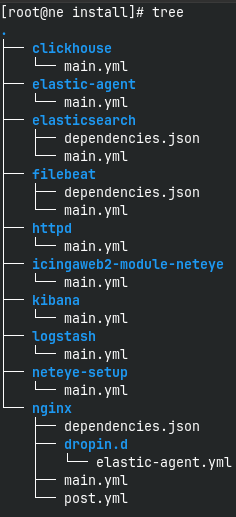
\includegraphics[width=.3\textwidth]{images/tree_install.png}
  \caption{Output del comando \texttt{tree} nella cartella della procedura di installazione}
  \label{fig:struttura_file_install}
\end{figure}\\ Quella appena presentata è solamente la parte iniziale della migrazione
degli script verso una procedura completamente parallelizzata ma risulta già possibile
notare un miglioramento, poiché il tempo necessario alla loro esecuzione prima
di queste modifiche era di circa due minuti, ora invece si è ridotto a circa venti
secondi.